% Created 2023-10-21 Sat 03:13
% Intended LaTeX compiler: pdflatex
\documentclass[11pt]{article}
\usepackage[utf8]{inputenc}
\usepackage[T1]{fontenc}
\usepackage{graphicx}
\usepackage{longtable}
\usepackage{wrapfig}
\usepackage{rotating}
\usepackage[normalem]{ulem}
\usepackage{amsmath}
\usepackage{amssymb}
\usepackage{capt-of}
\usepackage{hyperref}
\usepackage{graphicx}
\graphicspath{ {./images/} }
\author{Hankertrix}
\date{\today}
\title{Physics Electric Fields Tutorial}
\hypersetup{
 pdfauthor={Hankertrix},
 pdftitle={Physics Electric Fields Tutorial},
 pdfkeywords={},
 pdfsubject={},
 pdfcreator={Emacs 29.1 (Org mode 9.6.6)}, 
 pdflang={English}}
\begin{document}

\maketitle
\setcounter{tocdepth}{2}
\tableofcontents

\newpage

\section{Question 1}
\label{sec:org6d9ca8e}

\subsection{Point 1}
\label{sec:orga79d299}
Finding the electric field at point 1:
\begin{align*}
\vec{E}_1 &= \vec{E}_{-q} + \vec{E}_{+2q} \\
&= \frac{1}{4 \pi \varepsilon_0} \frac{q}{\sqrt{a^2 + 2a^2}^2} \frac{-\hat{i} - 2\hat{j}}{\sqrt{2^2 + 1^2}} + \frac{1}{4 \pi \varepsilon_0} \frac{2q}{\sqrt{a^2 +2a^2}^2} \frac{-\hat{i} + 2\hat{j}}{\sqrt{2^2 + 1^2}} \\
&= \frac{1}{4 \pi \varepsilon_0} \left( \frac{q(- \hat{i} - 2 \hat{j})}{5a^2 \cdot \sqrt{5}} + \frac{q( -2 \hat{i} + 4 \hat{j})}{5a^2 \cdot \sqrt{5}} \right) \\
&= \frac{1}{4 \pi \varepsilon_0} \left( \frac{q(- \hat{i} - 2 \hat{j} - 2 \hat{i} + 4 \hat{j})}{5 \sqrt{5} a^2} \right) \\
&= \frac{1}{4 \pi \varepsilon_0} \left( \frac{q(-3 \hat{i} + 2 \hat{j})}{5 \sqrt{5} a^2} \right) \\
&= \frac{1}{4 \pi \varepsilon_0} \left( \frac{q}{5 \sqrt{5} a^2} \right) (-3 \hat{i} + 2 \hat{j}) \\
\end{align*}

\subsection{Point 2}
\label{sec:org1bdfe82}
Finding the electric field at point 2:
\begin{align*}
\vec{E}_2 &= \vec{E}_{-q} + \vec{E}_{+2q} \\
&= \frac{1}{4 \pi \varepsilon_0} \frac{q}{a^2} \hat{i} + \frac{1}{4 \pi \varepsilon_0} \frac{2q}{(3a)^2} \cdot - \hat{i} \\
&= \frac{1}{4 \pi \varepsilon_0} \left( \frac{q}{a^2} - \frac{2q}{9a^2} \right) \hat{i} \\
&= \frac{1}{4 \pi \varepsilon_0} \left( \frac{9q}{9a^2} - \frac{2q}{9a^2} \right) \hat{i} \\
&= \frac{1}{4 \pi \varepsilon_0} \left( \frac{7q}{9a^2} \right) \hat{i} \\
\end{align*}

\newpage

\subsection{Neutral point}
\label{sec:org9c43e57}
The neutral point must be somewhere along the x-axis in between the 2 charges.
\\[0pt]

Let \(x\) be the distance of the neutral point from charge \(-q\):
\begin{align*}
\vec{E} &= \vec{E}_{-q} + \vec{E}_{+2q} \\
0 &= \frac{1}{4 \pi \varepsilon_0} \frac{q}{x^2} \cdot -\hat{i} + \frac{2q}{(2a - x)^2} \hat{i} \\
0 &= -\frac{1}{x^2} + \frac{2}{(2a - x)^2} \\
\frac{1}{x^2} &= \frac{2}{(2a - x)^2} \\
2a - x^2 &= 2x^2 \\
3x^2 &= 2a \\
x^2 &= \frac{2}{3} a \\
x &= \pm \sqrt{\frac{2}{3} a} \\
x &= \sqrt{\frac{2}{3} a} \quad (\because x > 0) \\
\end{align*}

The neutral point will be \(\sqrt{\frac{2}{3}a}\) away from the charge \(-q\).

\newpage


\section{Question 2}
\label{sec:org13cb2c8}
When the charges on the spheres are in equilibrium, the electric potential of both will be equal:
\[V_1 = V_2\]
\[\frac{1}{4 \pi \varepsilon_0} \frac{q_1}{r_1} = \frac{1}{4 \pi \varepsilon_0} \frac{q_2}{r_2}\]
\[\frac{q_1}{r_1} = \frac{q_2}{r_2}\]
\[\frac{r_2}{r_1} = \frac{q_2}{q_1}\]
\[q_2 = \frac{q_1 r_2}{r_1}\]

Finding the ratio of \(E_1\) to \(E_2\):
\begin{align*}
\frac{E_1}{E_2} &= \frac{1}{4 \pi \varepsilon_0} \frac{q_1}{r_1^2} \div \frac{1}{4 \pi \varepsilon_0} \frac{q_2}{r_2^2} \\
&= \frac{q_1}{r_1^2} \cdot \frac{r_2^2}{q_2} \\
&= \frac{q_1}{r_1^2} \cdot \frac{r_2^2}{q_1 \frac{r_2}{r_1}} \\
&= \frac{q_1}{r_1^2} \cdot \frac{r_2^2 r_1}{q_1 r_2} \\
&= \frac{r_2}{r_1} \\
\end{align*}

\newpage

\section{Question 3}
\label{sec:orgb09afec}
An expression for electric potential:
\[V = \frac{1}{4 \pi \varepsilon_0} \frac{q}{r}\]

Finding the work done, which is the potential energy, using potential:
\[W = \int_0^Q \frac{1}{4 \pi \varepsilon_0} \frac{q}{R} \, dq\]
\[W = \frac{1}{4 \pi \varepsilon_0 R} \int_0^Q q \, dq\]
\[W = \frac{1}{4 \pi \varepsilon_0 R} \left[\frac{q^2}{2} \right]_0^Q\]
\[W = \frac{1}{4 \pi \varepsilon_0 R} \left[\frac{Q^2}{2} - \frac{0}{2} \right]\]
\[W = \frac{1}{4 \pi \varepsilon_0 R} \frac{Q^2}{2}\]
\[W = \frac{Q^2}{8 \pi \varepsilon_0 R}\]

\newpage

\section{Question 4}
\label{sec:orgb1f1a60}

\subsection{(a)}
\label{sec:org5418a99}
Let \(\phi\) be the angle between \(r\) and \(\sqrt{r^2 + h^2}\).
\\[0pt]

Using the principle of linear super position for continuous charge distribution:
\[E = \int \frac{1}{4 \pi \varepsilon_0 \sqrt{h^2 + r^2}^2} \, dq \cdot \sin \phi\]
\[E = \int \frac{1}{4 \pi \varepsilon_0 (h^2 + r^2)} \, dq \cdot \sin \phi\]
\[E = \int \frac{1}{4 \pi \varepsilon_0 (h^2 + r^2)} \sigma \, dA \cdot \sin \phi \quad (\because dq = \sigma \, dA)\]
\[E = \int \frac{1}{4 \pi \varepsilon_0 (h^2 + r^2)} \sigma \cdot \delta r \cdot r \, d \theta \cdot \sin \phi \quad (\because dA = \delta r \cdot r \, d \theta)\]
\[E = \frac{\sigma r \delta r}{4 \pi \varepsilon_0 (h^2 + r^2)} \int 1 \, d \theta \cdot \sin \phi\]
\[E = \frac{\sigma r \delta r}{4 \pi \varepsilon_0 (h^2 + r^2)} \int_0^{2\pi} 1 \, d \theta \cdot \sin \phi\]
\[E = \frac{\sigma r \delta r}{4 \pi \varepsilon_0 (h^2 + r^2)} [\theta]_0^{2\pi} \cdot \sin \phi\]
\[E = \frac{\sigma r \delta r}{4 \pi \varepsilon_0 (h^2 + r^2)} [2 \pi - 0] \cdot \sin \phi\]
\[E = \frac{2 \pi \sigma r \delta r}{4 \pi \varepsilon_0 (h^2 + r^2)} \cdot \sin \phi\]
\[E = \frac{\sigma r \delta r}{2 \varepsilon_0 (h^2 + r^2)} \cdot \sin \phi\]
\[E = \frac{\sigma r \delta r}{2 \varepsilon_0 (h^2 + r^2)} \cdot \frac{h}{\sqrt{h^2 + r^2}}\]
\[E = \frac{\sigma r \delta r h}{2 \varepsilon_0 (h^2 + r^2)^{\frac{3}{2}}}\]

\newpage

The electric force would be:
\[F = qE\]
\[F = q \frac{\sigma r \delta r h}{2 \varepsilon_0 (h^2 + r^2)^{\frac{3}{2}}}\]
\[F = \frac{q \sigma r \delta r h}{2 \varepsilon_0 (h^2 + r^2)^{\frac{3}{2}}} \textbf{ (Shown)}\]

\subsection{(b)}
\label{sec:orgd256e5e}
The electric field of a large flat circular sheet would be the sum of all circular rings that eventually build up to a circular sheet.
\\[0pt]

Let \(\delta r\) be infinitesimally small, i.e. \(\delta r = dr\). Using the electric field in part \((a)\):
\[E = \int \frac{\sigma r h}{2 \varepsilon_0 (h^2 + r^2)^{\frac{3}{2}}} \, dr\]

Let \(\theta\) be the angle between \(h\) and \(\sqrt{h^2 + r^2}\).
\[\tan \theta = \frac{r}{h}\]
\[r = h \tan \theta\]
\[\frac{dr}{d \theta} = h \sec^2 \theta\]
\[dr = h \sec^2 \theta \, d \theta\]

Using the above substitutions, the electric field would be:
\begin{align*}
E &= \int \frac{\sigma h \tan \theta h}{2 \varepsilon_0 (h^2 + (h \tan \theta)^2)^{\frac{3}{2}}} \, h \sec^2 \theta \, d \theta \\
&= \frac{\sigma}{2 \varepsilon_0} \int \frac{h^3 \tan \theta}{(h^2 + h^2 \tan^2 \theta )^{\frac{3}{2}}} \, \sec^2 \theta \, d \theta \\
&= \frac{\sigma}{2 \varepsilon_0} \int \frac{h^3 \tan \theta}{(h^2(1 + \tan^2 \theta ))^{\frac{3}{2}}} \, \sec^2 \theta \, d \theta \\
&= \frac{\sigma}{2 \varepsilon_0} \int \frac{h^3 \tan \theta}{(h^2(1 + \tan^2 \theta ))^{\frac{3}{2}}} \, \sec^2 \theta \, d \theta \\
&= \frac{\sigma}{2 \varepsilon_0} \int \frac{h^3 \tan \theta}{h^3(1 + \tan^2 \theta)^{\frac{3}{2}}} \, \sec^2 \theta \, d \theta \\
&= \frac{\sigma}{2 \varepsilon_0} \int \frac{\tan \theta}{(1 + \tan^2 \theta)^{\frac{3}{2}}} \, \sec^2 \theta \, d \theta \\
&= \frac{\sigma}{2 \varepsilon_0} \int \frac{\sec^2 \theta \tan \theta}{(1 + \tan^2 \theta)^{\frac{3}{2}}} \, d \theta \\
&= \frac{\sigma}{2 \varepsilon_0} \int \sec^2 \theta \tan \theta (1 + \tan^2 \theta)^{-\frac{3}{2}} \, d \theta \\
&= \frac{\sigma}{2 \varepsilon_0} \int_0^{\frac{\pi}{2}} \frac{1}{2} \cdot 2 \sec^2 \theta \tan \theta (1 + \tan^2 \theta)^{-\frac{3}{2}} \, d \theta \\
&= \frac{\sigma}{2 \varepsilon_0} \left[\frac{1}{2} \cdot \frac{1}{-\frac{1}{2}} (1 + \tan^2 \theta)^{-\frac{1}{2}} \right]_0^{\frac{\pi}{2}} \\
&= \frac{\sigma}{2 \varepsilon_0} \left[\frac{1}{2} \cdot -2 (\sec^2 \theta)^{-\frac{1}{2}} \right]_0^{\frac{\pi}{2}} \\
&= \frac{\sigma}{2 \varepsilon_0} \left[-|\sec \theta|^{-1} \right]_0^{\frac{\pi}{2}} \\
&= \frac{\sigma}{2 \varepsilon_0} \left[-|\cos \theta| \right]_0^{\frac{\pi}{2}} \\
&= \frac{\sigma}{2 \varepsilon_0} \left[-\left|\cos \frac{\pi}{2} \right| - (-|\cos 0|) \right] \\
&= \frac{\sigma}{2 \varepsilon_0} [0 - (-1)] \\
&= \frac{\sigma}{2 \varepsilon_0} [1] \\
&= \frac{\sigma}{2 \varepsilon_0} \textbf{ (Shown)} \\
\end{align*}


\section{Question 5}
\label{sec:org64993df}
Using the definition of Gauss' Law:
\[\Phi = \frac{Q_{encl}}{\varepsilon_0}\]

Electric flux through S1:
\begin{align*}
\Phi_{S1} &= \frac{-2Q + Q}{\varepsilon_0} \\
&= \frac{-Q}{\varepsilon_0}
\end{align*}

Electric flux through S2:
\begin{align*}
\Phi_{S2} &= \frac{Q - Q}{\varepsilon_0} \\
&= 0
\end{align*}

Electric flux through S3:
\begin{align*}
\Phi_{S3} &= \frac{-2Q + Q - Q}{\varepsilon_0} \\
&= \frac{-3Q}{\varepsilon_0}
\end{align*}

Electric flux through S4:
\begin{align*}
\Phi_{S4} &= \frac{0}{\varepsilon_0} \\
&= 0
\end{align*}


\section{Question 6}
\label{sec:orgeaf5621}

\subsection{(a)}
\label{sec:org48914ba}
Using Gauss' Law:
\begin{align*}
\oint \vec{E} \cdot d \vec{A} &= \frac{Q_{encl}}{\varepsilon_0} \\
-15000 \cdot 4 \pi (8 \cdot 10^{-2})^2 &= \frac{Q_{encl}}{8.85 \cdot 10^{-12}} \quad (\because E \text{ is pointing inwards}) \\
Q_{encl} &= -1.067638847 \cdot 10^{-9} \\
Q_{encl} &\approx -1.07 \cdot 10^{-9} \\
\end{align*}

\subsection{(b)}
\label{sec:orgf2e3d26}
Using Gauss' Law:
\begin{align*}
\oint \vec{E} \cdot d \vec{A} &= \frac{Q_{encl}}{\varepsilon_0} \\
15000 \cdot 4 \pi (8 \cdot 10^{-2})^2 &= \frac{Q_{encl}}{8.85 \cdot 10^{-12}} \quad (\because E \text{ is pointing outwards}) \\
Q_{encl} &= 1.067638847 \cdot 10^{-9} \\
Q_{encl} &\approx 1.07 \cdot 10^{-9} \\
\end{align*}

\subsection{(c)}
\label{sec:orgd8ffcfb}
Using Gauss' Law:
\begin{align*}
\oint \vec{E} \cdot d \vec{A} &= \frac{Q_{encl}}{\varepsilon_0} \\
15000 \cdot 4 \pi (17 \cdot 10^{-2})^2 &= \frac{Q_{encl}}{8.85 \cdot 10^{-12}} \quad (\because E \text{ is pointing outwards}) \\
Q_{encl} &= 4.82105667 \cdot 10^{-9} \\
Q_{encl} &\approx 4.82 \cdot 10^{-9} \\
\end{align*}


\section{Question 7}
\label{sec:org0ce7da7}

\subsection{(a)}
\label{sec:org78294b6}
\[\tau = \vec{F} \times \vec{d}\]
\[\tau = q\vec{E} \times \vec{d}\]
\[\tau = \vec{E} \times q\vec{d}\]
\[\tau = \vec{E} \times \vec{p}\]
\[\tau = \vec{p} \times \vec{E} \textbf{ (Shown)}\]


\subsection{(b)}
\label{sec:orgde172ce}
\begin{align*}
\Delta U &= - \int \vec{F} \cdot \, d \vec{l} \\
&= - \int_{W_i}^{W_f} \, dW \\
&= - \int_{\theta_i}^{\theta_f} \tau \, d \theta \\
&= - \int_{\theta_i}^{\theta_f} pE \sin \theta \, d \theta \\
&= - [pE \cos \theta]_{\theta_i}^{\theta_f} \\
&= - [pE \cos \theta_f - pE \cos \theta_i ] \\
&= - pE(\cos \theta_f - \cos \theta_i) \textbf{ (Shown)} \\
\end{align*}


\section{Question 8}
\label{sec:org9e524b2}

\subsection{(a)}
\label{sec:org99ae30e}
The dipole moment in the \(y\) direction will cancel out, hence, the net dipole moment is:
\[p_{net} = p_1 \cos \theta + p_2 \cos \theta\]
\[p_{net} = \cos \theta (p_1 + p_2) \]

Using the definition of dipole moment:
\[p = qd\]
\[p_{net} = \cos \theta (qd + qd) \]
\[p_{net} = 2qd \cos \theta\]
\[6.1 \cdot 10^{-30} = (q \cdot 0.96 \cdot 10^{-10} + q \cdot 0.96 \cdot 10^{-10}) \cos 52^{\circ}\]
\[6.1 \cdot 10^{-30} = 2q \cdot 0.96 \cdot 10^{-10} \cdot \cos 52^{\circ}\]
\[q = 5.160438749 \cdot 10^{-20}\]
\[q \approx 5.16 \cdot 10^{-20}\]

\subsection{(b)}
\label{sec:orgbbc0911}
\[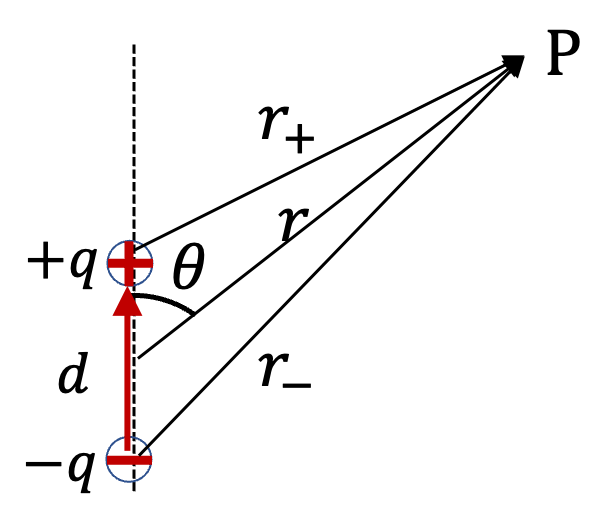
\includegraphics{dipole-potential-derivation}\]

The actual potential when adding up the two charges is:
\[V = \frac{q}{4 \pi \varepsilon_0 r_+} - \frac{q}{4 \pi \varepsilon_0 r_-}\]
\[V = \frac{q}{4 \pi \varepsilon_0} \left( \frac{1}{r_+} - \frac{1}{r_-} \right) \tag{1}\]

\newpage

\subsubsection{Finding an approximation for \(\frac{1}{r_+}\)}
\label{sec:org3efd564}
Using the law of cosines:
\[r_+^2 = r^2 + \left(\frac{d}{2} \right)^2 - 2r \frac{d}{2} \cos \theta\]
\[r_+^2 = r^2 + \left(\frac{d}{2} \right)^2 - rd \cos \theta\]
\[r_+^2 = r^2 + \frac{d^2}{4} - rd \cos \theta\]
\[r_+^2 = r^2 \left(1 + \frac{d^2}{4r^2} - \frac{d}{r} \cos \theta \right)\]
\[r_+^2 = r^2 \left(1 + \frac{1}{4} \left( \frac{d}{r} \right)^2 - \frac{d}{r} \cos \theta \right)\]
\[r_+^2 = r^2 \left(1 - \frac{d}{r} \cos \theta + \frac{1}{4} \left( \frac{d}{r} \right)^2 \right)\]
\[r_+ = r \left(1 - \frac{d}{r} \cos \theta + \frac{1}{4} \left( \frac{d}{r} \right)^2 \right)^{\frac{1}{2}}\]
\[\frac{1}{r_+} = \frac{1}{r} \left(1 - \frac{d}{r} \cos \theta + \frac{1}{4} \left( \frac{d}{r} \right)^2 \right)^{-\frac{1}{2}}\]
\[\frac{1}{r_+} = \frac{1}{r} \left(1 + \frac{1}{2} \frac{d}{r} \cos \theta - \frac{1}{8} \left(\frac{d}{r} \right)^2 + \frac{3}{8} \left( \frac{d}{r} \right)^2 \cos^2 \theta + \cdots \right)\]
\[\frac{1}{r_+} = \frac{1}{r} + \frac{1}{2} \frac{d}{r^2} \cos \theta - \frac{1}{8} \frac{d^2}{r^3} + \frac{3}{8} \frac{d^2}{r^3} \cos^2 \theta + \cdots \right)\]

When \(\frac{d}{r} << 1\), we can ignore the powers of \(\frac{d}{r}\) that are greater than 2:
\[\frac{1}{r_+} \approx \frac{1}{r} + \frac{1}{2} \frac{d}{r^2} \cos \theta \tag{2}\]

\newpage

\subsubsection{Finding an approximation for \(\frac{1}{r_-}\)}
\label{sec:org7ca3e7e}
Using the law of cosines:
\[r_-^2 = r^2 + \left(\frac{d}{2} \right)^2 - 2r \frac{d}{2} \cos (\pi - \theta)\]
\[r_-^2 = r^2 + \frac{d^2}{4} - rd \cos (\pi - \theta)\]
\[r_-^2 = r^2 + \frac{d^2}{4} + rd \cos \theta\]
\[r_-^2 = r^2 + rd \cos \theta + \frac{d^2}{4}\]
\[r_-^2 = r^2 \left(1 + \frac{d}{r} \cos \theta + \frac{d^2}{4r^2} \right)\]
\[r_-^2 = r^2 \left(1 + \frac{d}{r} \cos \theta + \frac{1}{4} \left( \frac{d}{r} \right)^2 \right)\]
\[r_- = r \left(1 + \frac{d}{r} \cos \theta + \frac{1}{4} \left( \frac{d}{r} \right)^2 \right)^{\frac{1}{2}}\]
\[\frac{1}{r_-} = \frac{1}{r} \left(1 + \frac{d}{r} \cos \theta + \frac{1}{4} \left( \frac{d}{r} \right)^2 \right)^{-\frac{1}{2}}\]
\[\frac{1}{r_-} = \frac{1}{r} \left(1 - \frac{1}{2} \frac{d}{r} \cos \theta - \frac{1}{8} \left( \frac{d}{r} \right)^2 - \frac{3}{8} \left( \frac{d}{r} \right)^2 \cos^2 \theta + \cdots \right)\]
\[\frac{1}{r_-} = \frac{1}{r} - \frac{1}{2} \frac{d}{r^2} \cos \theta - \frac{1}{8} \frac{d^2}{r^3} - \frac{3}{8} \frac{d^2}{r^3} \cos^2 \theta + \cdots\]

When \(\frac{d}{r} << 1\), we can ignore the powers of \(\frac{d}{r}\) that are greater than 2:
\[\frac{1}{r_-} \approx \frac{1}{r} - \frac{1}{2} \frac{d}{r^2} \cos \theta \tag{3}\]

\newpage

\subsubsection{Substituting the approximations back into the original equation}
\label{sec:org68fe7ed}
Substituting \((2)\) and \((3)\) into \((1)\):
\[V \approx \frac{q}{4 \pi \varepsilon_0} \left( \frac{1}{r} + \frac{1}{2} \frac{d}{r^2} \cos \theta - \left(\frac{1}{r} - \frac{1}{2} \frac{d}{r^2} \cos \theta \right) \right)\]
\[V \approx \frac{q}{4 \pi \varepsilon_0} \left( \frac{1}{r} + \frac{1}{2} \frac{d}{r^2} \cos \theta - \frac{1}{r} + \frac{1}{2} \frac{d}{r^2} \cos \theta \right)\]
\[V \approx \frac{q}{4 \pi \varepsilon_0} \left(\frac{1}{2} \frac{d}{r^2} \cos \theta + \frac{1}{2} \frac{d}{r^2} \cos \theta \right)\]
\[V \approx \frac{q}{4 \pi \varepsilon_0} \frac{d}{r^2} \cos \theta\]
\[V \approx \frac{qd \cos \theta}{4 \pi \varepsilon_0 r^2}\]

Since \(p = qd\):
\[V \approx \frac{p \cos \theta}{4 \pi \varepsilon_0 r^2}\]
\[V \approx \frac{1}{4 \pi \varepsilon_0} \frac{p \cos \theta}{r^2} \textbf{ (Shown)}\]
\end{document}